% Opsætter KU Tex dokument
%%%%%%%%%%%%%%%%%%%%%%%%%%%%%%%%%%%%%%%%%%%%%%%%%%%%%%%%%%%%%%%%%%%%%%%%%%%%%%%%
\documentclass{article}                                                        %
\usepackage[a4paper, hmargin={2.8cm, 2.8cm}, vmargin={2.5cm, 2.5cm}]{geometry} %
\usepackage{eso-pic}  % \AddToShipoutPicture                                   %
\usepackage{graphicx} % \includegraphics                                       %
%\usepackage{subfig} - Can not be used with subcaption package (for subfigures)
\usepackage{setspace}                                                        %
%%%%%%%%%%%%%%%%%%%%%%%%%%%%%%%%%%%%%%%%%%%%%%%%%%%%%%%%%%%%%%%%%%%%%%%%%%%%%%%%

% Pakker til skrifttyper, tekst osv.
%%%%%%%%%%%%%%%%%%%%%%%%%%%%%%%%%%%%%%%%%%%%%%%%%%%%%%%%%%%%%%%%%%%%%%%%%%%%%%%%
    \usepackage[utf8]{inputenc}  % Implementere Unicode                        %
    \usepackage[T1]{fontenc}     % Unicode skrifttype fx. é skrives som 1 tegn %
    \usepackage[english]{babel}   % Dansk Ordbog                                %
    \usepackage{microtype}       % Forbedre linjeombrydningen                  %
    \usepackage{libertine}       % Skrifttype                                  %
%%%%%%%%%%%%%%%%%%%%%%%%%%%%%%%%%%%%%%%%%%%%%%%%%%%%%%%%%%%%%%%%%%%%%%%%%%%%%%%%

% Pakker til matematik og kode.
%%%%%%%%%%%%%%%%%%%%%%%%%%%%%%%%%%%%%%%%%%%%%%%%%%%%%%%%%%%%%%%%%%%%%%%%%%%%%%%%
    \usepackage{mathtools}       % Udvidelse til amsmath pakken                %
    \usepackage{amsthm}          % Pakke til bevisførelse                      %
    \usepackage{amssymb}         % Extra matematiske symboler                  %				
	\usepackage{mychemistry}												   %
	\usepackage[version=3]{mhchem}											   %
	\usepackage{wrapfig}													   %
	\usepackage{siunitx}	
	\usepackage{anyfontsize}
	\usepackage{ragged2e}
	\usepackage{algorithm2e}
	\usepackage[final]{pdfpages}
	\usepackage{listings}
	\usepackage{tikz}
	\usepackage{multirow}
	\usepackage{makecell}
	\usepackage{fourier} 
	\usepackage{array}
	\usepackage{todonotes}
	\usepackage{pdflscape}
	\usetikzlibrary{arrows,shapes}
	\usepackage{titlesec}
	\usepackage{hyperref}
	\usepackage{url}
	\usepackage[nottoc,numbib]{tocbibind}
	\usepackage{semantic}
	\usepackage{subcaption}
	\usepackage{qtree}
	\usepackage{hhline}
	
	\definecolor{light-gray}{gray}{0.85}
	\lstset{
	    	numbers=left,
	    	breaklines=true,
	    	backgroundcolor=\color{light-gray},
	    	tabsize=2,
	    	basicstyle=\ttfamily,
	    	literate={\ \ }{{\ }}1
	}
	
	\urlstyle{same}
	\tikzstyle{vertex}=[circle,fill=white!25,minimum size=20pt,inner sep=0pt]
	\tikzstyle{edge} = [draw,thick,-]

	\definecolor{light-gray}{gray}{0.85}
	\definecolor{dkgreen}{RGB}{0.0,128.0,43.0}
	\lstdefinelanguage{FSharp}%
{morekeywords={new, match, with, rec, open, module, namespace, type, of, member, % 
and, for, while, true, false, in, do, begin, fun, function, return, yield, try, %end
mutable, if, then, else, cloud, async, static, use, abstract, interface, inherit, finally, int },
  otherkeywords={ let!, return!, do!, yield!, use!, var, from, select, where, order, by },
  keywordstyle=\color{bluekeywords},
  sensitive=true,
  basicstyle=\ttfamily,
	breaklines=true,
  xleftmargin=\parindent,
  aboveskip=\bigskipamount,
	tabsize=4,
  morecomment=[l][\color{dkgreen}]{///},
  morecomment=[l][\color{dkgreen}]{//},
  morecomment=[l][\color{dkgreen}]{(*},
  morecomment=[s][\color{dkgreen}]{},
  morestring=[b]",
  showstringspaces=false,
  literate={`}{\`}1,
  stringstyle=\color{redstrings},
}
	
	
												   %
%%%%%%%%%%%%%%%%%%%%%%%%%%%%%%%%%%%%%%%%%%%%%%%%%%%%%%%%%%%%%%%%%%%%%%%%%%%%%%%%

% Pakker til layout.
%%%%%%%%%%%%%%%%%%%%%%%%%%%%%%%%%%%%%%%%%%%%%%%%%%%%%%%%%%%%%%%%%%%%%%%%%%%%%%%%
    \usepackage{fancyhdr}            % Gør det muligt at bruge sidehoveder     %
    \usepackage{graphicx}            % Mulighed for bl.a. \includegraphics     %
    \usepackage{colortbl}            % Hvis man vil farvelægge sine tabeller   %
    \usepackage{array}               % Gør miljøerne array og tabular bedre    %
    \usepackage{parskip}             % Første paragraf i afsnit indrykkes ikke %
    \usepackage{titlesec}            % Tilpassing af afstand mellem sektioner  %
    \usepackage[lastpage,user]{zref} % Side x af y                             %
%%%%%%%%%%%%%%%%%%%%%%%%%%%%%%%%%%%%%%%%%%%%%%%%%%%%%%%%%%%%%%%%%%%%%%%%%%%%%%%%


% Implementerer en række makroer og de pakker der er importeret
%%%%%%%%%%%%%%%%%%%%%%%%%%%%%%%%%%%%%%%%%%%%%%%%%%%%%%%%%%%%%%%%%%%%%%%%%%%%%%%%
    \pagestyle{fancy}                        % Implementerer sidehoved         %
    \lhead{University of Copenhagen}                % Venstre sidehoved               %
    \rhead{Casper Bresdahl}                             % Højre sidehoved      %
    \cfoot{\thepage\ of \zpageref{LastPage}} % Side x af y                     %
    \newtheorem*{prp}{Propostion}            % Skaber nyt theorem  
    \renewcommand{\baselinestretch}{1.25}       %
%%%%%%%%%%%%%%%%%%%%%%%%%%%%%%%%%%%%%%%%%%%%%%%%%%%%%%%%%%%%%%%%%%%%%%%%%%%%%%%%

% Mindsker afstanden mellem sektioner
%%%%%%%%%%%%%%%%%%%%%%%%%%%%%%%%%%%%%%%%%%%%%%%%%%%%%%%%%%%%%%%%%%%%%%%%%%%%%%%%%%
\titlespacing\section{0pt}{12pt plus 4pt minus 2pt}{0pt plus 1pt minus 3pt}      %
\titlespacing\subsection{0pt}{12pt plus 4pt minus 2pt}{0pt plus 1pt minus 3pt}   %
\titlespacing\subsubsection{0pt}{12pt plus 4pt minus 2pt}{0pt plus 1pt minus 3pt}%
%%%%%%%%%%%%%%%%%%%%%%%%%%%%%%%%%%%%%%%%%%%%%%%%%%%%%%%%%%%%%%%%%%%%%%%%%%%%%%%%%%

%Ændrer størelsen på sections
%%%%%%%%%%%%%%%%%%%%%%%%%%%%%%%%%%%%%%%%%%%%%%%%%%%%%%%%%%%%%%%%%%%%%%%%%%%%%%%%%%
\titleformat{\section}
{\normalfont\fontsize{14}{16}\bfseries}{\thesection}{1em}{}
\titleformat{\subsection}
{\normalfont\fontsize{12}{14}\bfseries}{\thesubsection}{1em}{}
\titleformat{\subsubsection}
{\normalfont\fontsize{11}{13}\bfseries}{\thesubsubsection}{1em}{}
%%%%%%%%%%%%%%%%%%%%%%%%%%%%%%%%%%%%%%%%%%%%%%%%%%%%%%%%%%%%%%%%%%%%%%%%%%%%%%%%%%

%%%%%%%%%%%%
% Document %
%%%%%%%%%%%%

\begin{document}

\begin{titlepage}

\newcommand{\HRule}{\rule{\linewidth}{0.5mm}} % Defines a new command for the horizontal lines, change thickness here

\begin{center}
 % Center everything on the page
 
%----------------------------------------------------------------------------------------
%	HEADING SECTIONS
%----------------------------------------------------------------------------------------

\textsc{\LARGE University of Copenhagen}\\[1.5cm] % Name of your university/college
\textsc{\Large Computer Science}\\[0.5cm] % Major heading such as course name
\textsc{\large Advanced Topics in Image Analysis}\\[0.5cm] % Minor heading such as course title

%----------------------------------------------------------------------------------------
%	TITLE SECTION
%----------------------------------------------------------------------------------------

\HRule \\[0.4cm]
{ \huge \bfseries Assignment 3}\\[0.4cm] % Title of your document
\HRule \\[1.5cm]
 
%----------------------------------------------------------------------------------------
%	AUTHOR SECTION
%----------------------------------------------------------------------------------------

\begin{minipage}{0.4\textwidth}
\begin{flushleft} \large
\emph{Author:}\\ 
% Your name
Casper \textsc{Bresdahl} \\
\end{flushleft}
\end{minipage}
~
\begin{minipage}{0.4\textwidth}
\begin{flushright} \large
\emph{Teacher:} \\
Sune \textsc{Darkner}
\end{flushright}
\end{minipage}\\[2cm]

% If you don't want a supervisor, uncomment the two lines below and remove the section above
%\Large \emph{Forfattere:}\\
%Axel \textsc{Christof}\\% Your name
%Casper \textsc{Bresdahl}\\
%Emilie \textsc{Bentsen}\\[1cm] 

%----------------------------------------------------------------------------------------
%	DATE SECTION
%----------------------------------------------------------------------------------------

{\large \today}\\[2cm] % Date, change the \today to a set date if you want to be precise

%----------------------------------------------------------------------------------------
%	LOGO SECTION
%----------------------------------------------------------------------------------------


\includegraphics{logo.png}\\[1cm] % Include a department/university logo - this will require the graphicx package
 
%----------------------------------------------------------------------------------------

\vfill % Fill the rest of the page with whitespace

%Disse linjer skaber forside, evt indholdsfortegnelse, og sætter sidetal
%%%%%%%%%%%%%%%%%%%%%%%%%%%%%%%%%%%%%%%%%%%%%%%%%%%%%%%%%%%%%%%%%%%%%%%%%%%%%%%%
									                                           %
    \thispagestyle{empty}   % Fjerner sidetal forside                          %
        % Slå disse til hvis der ønskes indholdsfortegnelse                    %
        %%%%%%%%%%%%%%%%%%%%%%%%%%%%%%%%%%%%%%%%%%%%%%%%%%%%%%%%%%%%%%%%%%%%%%%% 
            \newpage                % Side til indholdsfortegnelse            %
            %\thispagestyle{empty}   % Fjerner sidetal fra indholdsfortegnelse %
            %\tableofcontents        % Skaber indholdsfortegnelse              %
    \end{center}
    %\section*{Forord}
    	
		
        %%%%%%%%%%%%%%%%%%%%%%%%%%%%%%%%%%%%%%%%%%%%%%%%%%%%%%%%%%%%%%%%%%%%%%%%
    \newpage                % Første rigtige side
    \setcounter{page}{1}    % Sætter rigtigt sidetal på første side
%%%%%%%%%%%%%%%%%%%%%%%%%%%%%%%%%%%%%%%%%%%%%%%%%%%%%%%%%%%%%%%%%%%%%%%%%%%%%

\end{titlepage}
{\fontsize{10}{14}\selectfont
\section{Assignment 3}

\subsection{Design of experiments}
%When comparing images taken of the same scene, three common changes are scale, rotation and illumination. Because of this, I have designed my experiments to evaluate image descriptors on a roughly equal amount of images mainly varying in scale, rotation and illumination. 
For this assignment a subset of the 'HPatches' data set has been chosen, namely the first 10 series with illumination changes and the 10 fist series with view point changes. Three image descriptors, namely SIFT, ORB and SURF will then be evaluated on the aforementioned data. A consideration for the experiments have been, that an image descriptor both chooses a location in an image which it finds fitting, and it describes this location. That is, we both get key points and descriptors for each found feature in the image. To evaluate the key points we use \textit{mean localization error}, to evaluate descriptors we use \textit{nearest neighbour mean average precision}, and to evaluate the image descriptor as a whole, we use \textit{homography estimation}. Before going into details with these error measures, we will first look at how we classify true positives, false positives and false negative detections.\\
For each pair of images considered, we apply the image descriptor to both images, and the detections made in \textit{image 1} are considered ground truth whereas the detections made in \textit{image 2} are considered candidate points. If there is a perspective change between the two images, the ground truths are warped into the perspective of the candidate points. To detect false positives, we go through each detection in our candidate points, and each candidate point which does not have a similar ground truth is considered a false positive. To detect false negatives we go through each ground truth and if it does not have a similar candidate point it is a false negative. A true positive can be measured as either each candidate point which has a similar ground truth, or each ground truth which has a similar candidate point. This 'similar' / $\epsilon$ term is measured as the L2 norm, and can be increased / shrunk in order to create precision / recall curves. We will compute precision and recall by starting with $\epsilon = 0$ and increase it.
As we might have more ground truths than candidate points and vice versa, the recall and precision is rescaled to always go from 0 to 1. 
To ensure correct curves, 1 - recall will be used to compute precision / recall curves. An example of a precision / recall curve can be seen in \autoref{PRCurve}. Each ground truth or candidate point can only be matched once, that is, if we have two candidate points around a ground truth, only one of them will be considered a true positive whereas the other will be considered a false positive.\\
\textit{opencv} implementations of the image descriptors have been used, and all image descriptors have their default parameters.

\begin{figure}[h]
	\centering
	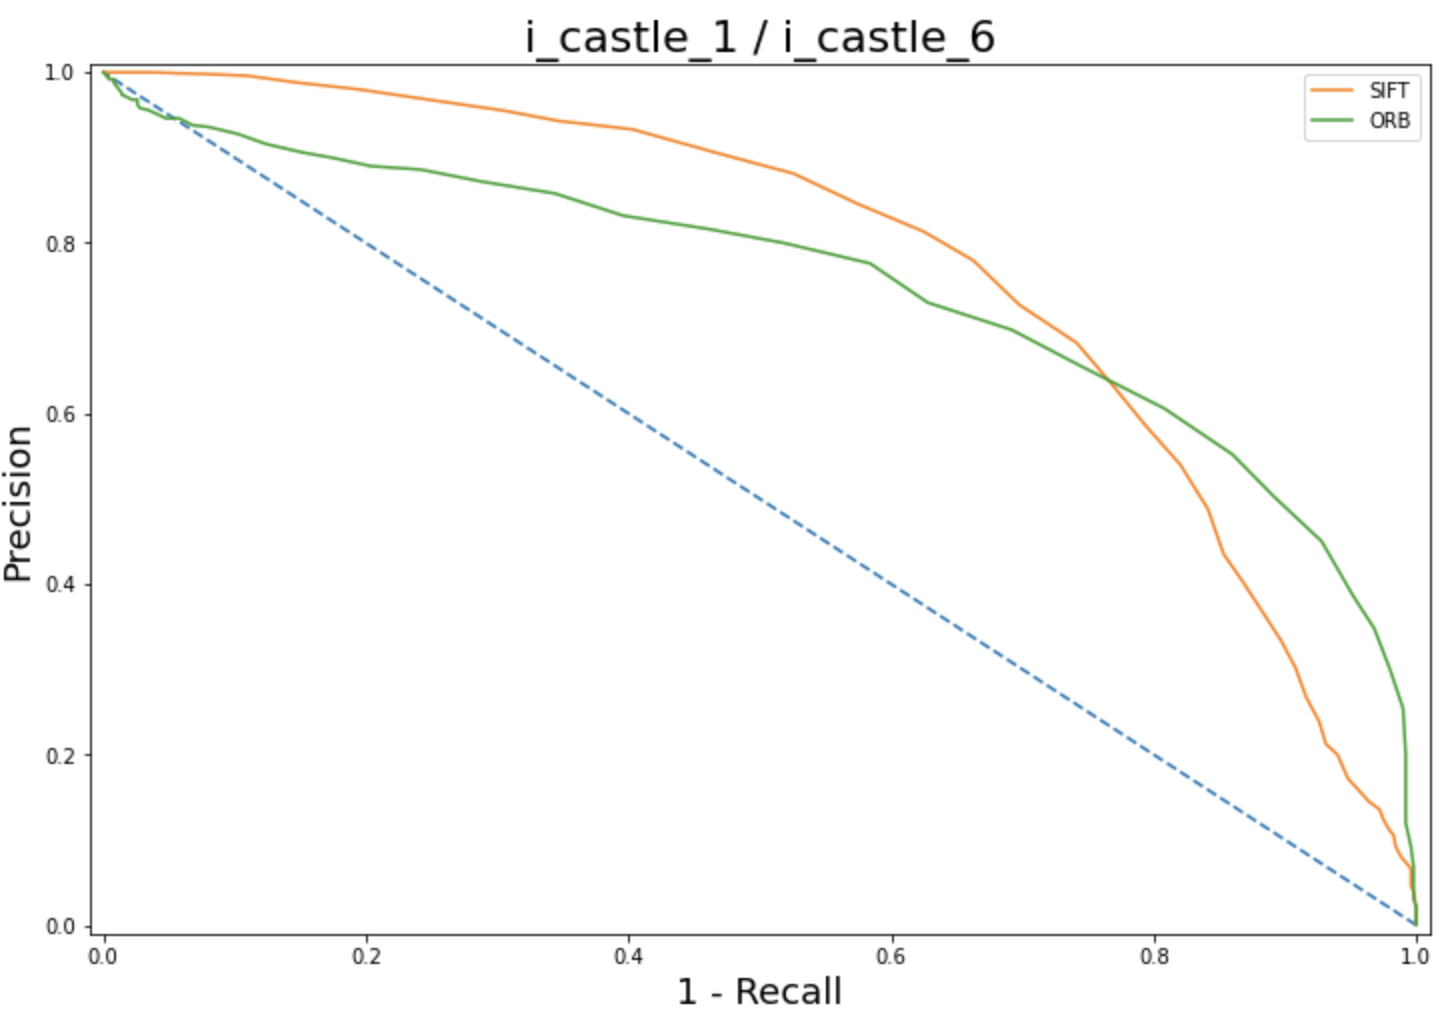
\includegraphics[width=0.68\linewidth]{Materials/PRCurve}
	\caption{Precision / recall curve for two images in the castle series.}
	\label{PRCurve}
\end{figure}
\subsection{Error measures}
We can now discuss the definition of each error measure.\\
\textit{Mean localization error} is defined in accordance to \cite{sp} where we only use true positive detections and find the average distance between their nearest neighbours. This measure tells us about how close the key points are to each other in the two images, that is, if the image descriptor finds the same points in the two images. The error ranges between 0 and $\epsilon$, where $\epsilon$ is the maximum distance between the two key points there can be for them to be considered true positives. As it is unclear which epsilon is used in \cite{sp}, I have chosen to report the mean localization error for a range of epsilon values. To avoid rewarding image descriptors which find 0 features, the maximum error ($\epsilon$) is used for a run where 0 features are found.\\
\textit{Nearest neighbour mean average precision} is defined in accordance to \cite{sp}, and takes all descriptors of an image pair and finds their nearest neighbour. Then creates a precision / recall curve and measures the area under the curve for this image pair. Then the average area under the curve is estimated across all image pairs. This measure estimates how well the image descriptor detects true positives without introducing false positives. The measure ranges between 0 and 1. As we are comparing the same scene, the descriptions made should describe the same image patches, and thus we do not perform any perspective warping for this measure. As it is not clear from \cite{sp} which range of $\epsilon$ values are used, I have chosen to use 100 evenly spaced $\epsilon$ values between 100 - 800 as the distance between all found descriptors in the manually inspected images seem to be matched in this range. To make this measure computational feasible, only the first 1000 descriptors found are used. These are likely in the same part of the image, but sampling 1000 descriptors across the image might result in a lot of descriptors which are not measured at the same key points.\\
\textit{Homography estimation} is defined in accordance to \cite{sp} and takes the four corners of \textit{image 1} and first measures the average distance between each corresponding corner transformed by the true homography matrix and the estimated homography matrix found by taking nearest neighbour matches found by the image descriptor. If the average distance is less than some $\epsilon$ then it is reported as a correct homography estimation, otherwise it is reported as a wrong estimation. The average number of correct estimations over all image pairs is then reported as the \textit{homography estimation} measure. This measure evaluates the image descriptor as a whole by taking points matched in the two images to estimate a homography to warp one image into the perspective of the other. The result ranges between 0 and 1. As SIFT returns \textit{a lot} of features, a Lowe's ratio at $0.7$ is used to filter the number of features used to estimate the homography.
\subsection{Results}
To get an idea of how many features each image descriptor produces, we will begin this section by taking a look at three image pairs where each image descriptor have been run. The found features can be seen in \autoref{noFeatures}, and only shows correct correspondences. By manual inspection, it can also be reported that in general (when not constrained) SIFT and SURF produces more matches than ORB.

\begin{figure}[h]
	\centering
	\begin{subfigure}{0.8\linewidth}
		\centering
		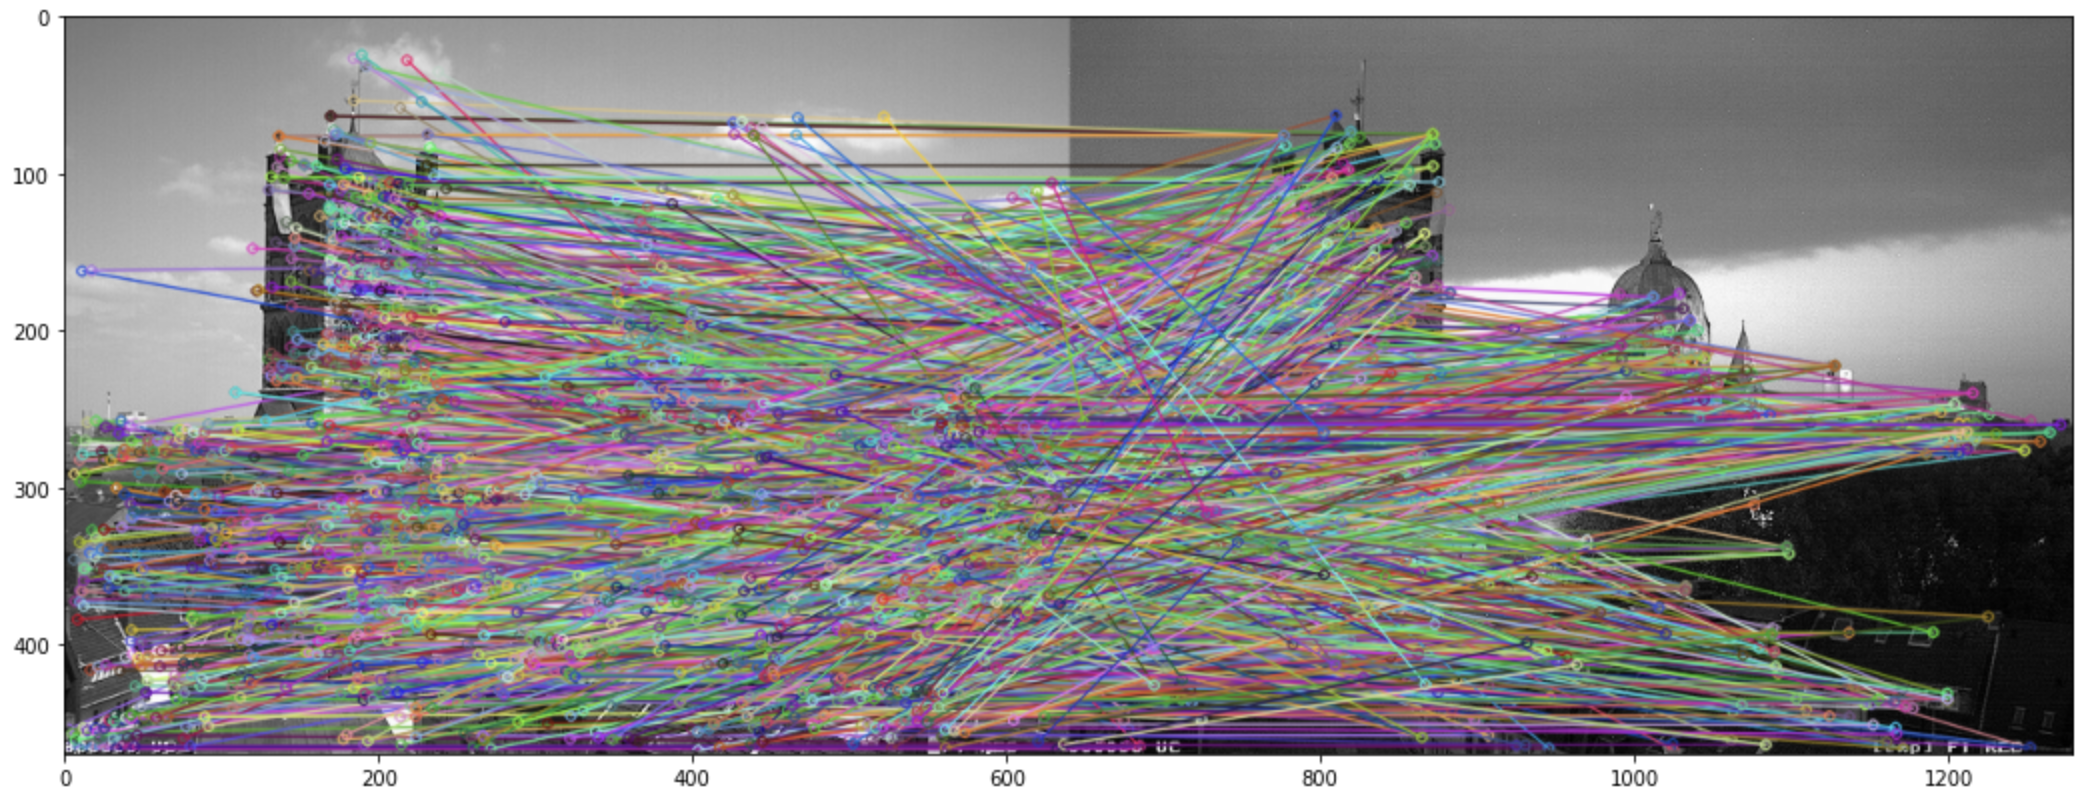
\includegraphics[width=\linewidth]{Materials/SIFTMatches}
		\caption{The detected SIFT features.}
	\end{subfigure}
	\\
	\begin{subfigure}{0.8\linewidth}
		\centering
		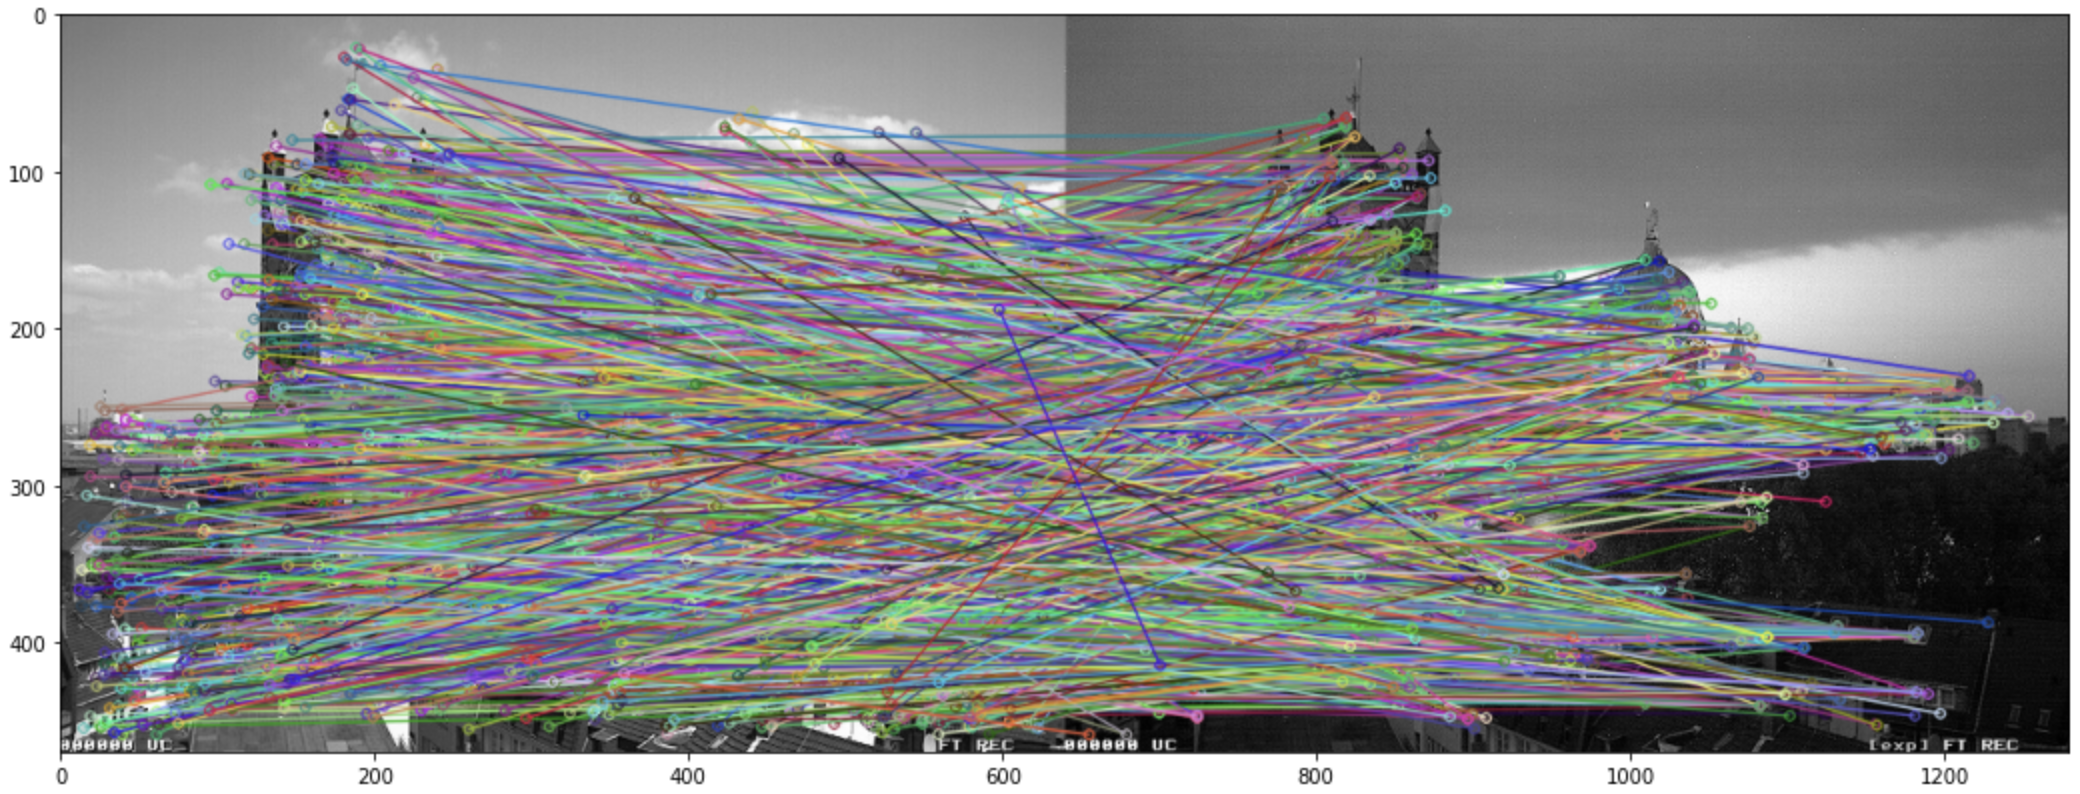
\includegraphics[width=\linewidth]{Materials/SURFMatches}
		\caption{The detected SURF features.}
	\end{subfigure}
	\\
	\begin{subfigure}{0.8\linewidth}
		\centering
		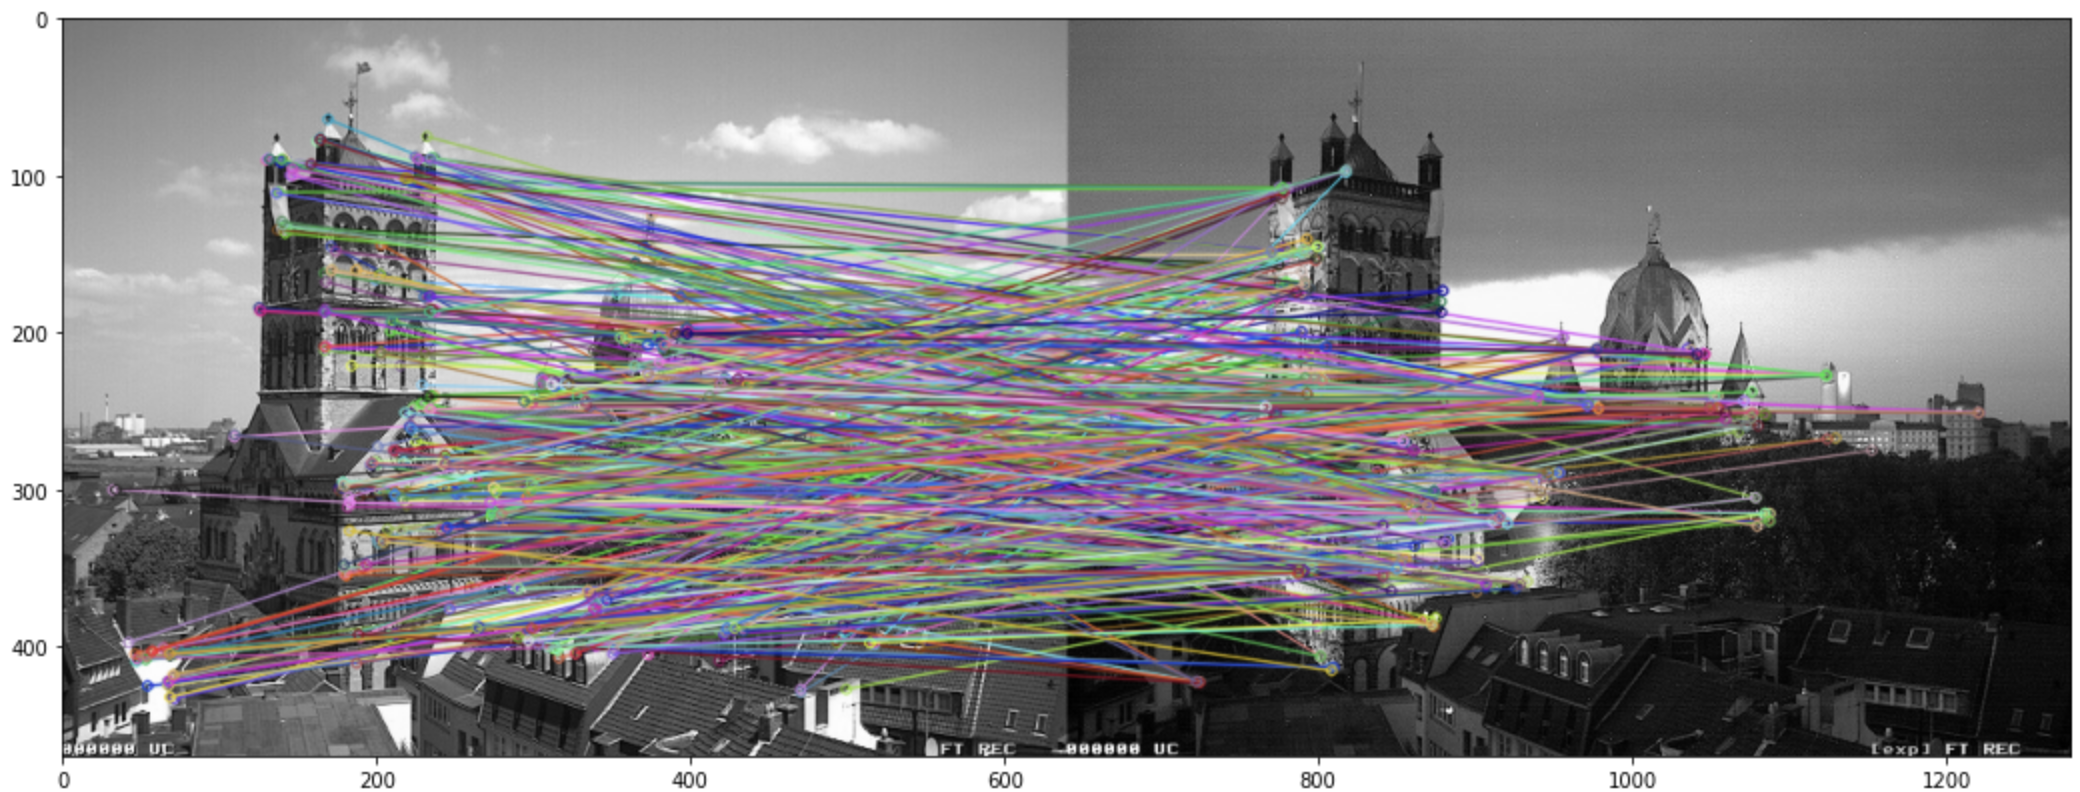
\includegraphics[width=\linewidth]{Materials/ORBMatches}
		\caption{The detected ORB features.}
	\end{subfigure}
	\caption{Each image descriptor run on the same image pair to give an indication of how many features each finds.}
	\label{noFeatures}
\end{figure}

\begin{table}[h]
	\centering
	\begin{tabular}{|c||ccc||ccc||c|}
		\hline
		& \multicolumn{3}{c||}{Homography estimation}                           & \multicolumn{3}{c||}{Mean localization error}                          & NN mean average precision \\ \hline
		& \multicolumn{1}{c|}{eps = 1} & \multicolumn{1}{c|}{eps = 3} & eps = 5 & \multicolumn{1}{c|}{eps = 1} & \multicolumn{1}{c|}{eps = 3} & eps = 5 &                           \\ \hline
		SIFT & \multicolumn{1}{c|}{0.34}   & \multicolumn{1}{c|}{0.61}    & 0.71    & \multicolumn{1}{c|}{0.56}    & \multicolumn{1}{c|}{1.46}    & 2.41    & 0.72                      \\ \hline
		ORB  & \multicolumn{1}{c|}{0.05}   & \multicolumn{1}{c|}{0.21}    & 0.31    & \multicolumn{1}{c|}{0.54}    & \multicolumn{1}{c|}{1.54}    & 2.41    & 0.73                      \\ \hline
		SURF & \multicolumn{1}{c|}{0.29}   & \multicolumn{1}{c|}{0.53}    & 0.66    & \multicolumn{1}{c|}{0.56}    & \multicolumn{1}{c|}{1.48}    & 2.27    & 0.50                      \\ \hline
	\end{tabular}
	\caption{Results of the experiments.}
	\label{results}
\end{table}
As seen, SIFT finds about as many features as SURF whereas ORB finds a considerable amount less.\\
In \autoref{results} we see the results of the experiments conducted. When comparing SIFT and ORB we see their ability to estimate correct homographies varies greatly. ORB estimates as many correctly homographies when epsilon is 5 as SIFT does when epsilon is 1, that is, SIFT is much more accurate when estimating homographies. SURF lies in between the two, performing closer to SIFT than ORB. However, when we compare the mean localization error SIFT, SURF and ORB obtain similar errors. This means their ability to choose the same places in the image pairs are equivalent. However, looking at the actual errors, we see the error is about halfway between the minimum and maximum possible which means we are fairly far away from the actual location we were looking for. When it comes to nearest neighbour mean average precision SIFT and ORB performs similar and fairly well, whereas SURF performs quite poorly.
\subsection{Discussion of results}
A reason for the big difference in homography estimation performance between SIFT and ORB might be how many feature points each find and are able to match. SIFT does find a considerable amount more features than ORB does, and because SIFT have more points, and point matches, it is able to estimate the homography better. RANSAC is used to eliminate outliers, which means even though SIFT might find more false positive matches, some are eliminated. It is likely SURF performs better than ORB for the same reason, however, because SURF produces worse descriptors (seen from nearest neighbour mean average precision) than SIFT, it is worse at estimating the homographies than SIFT.\\
The fact the mean localization error seems to be fairly high for all image descriptors might be due some aliasing or other approximation of the new location after moving the ground truth point locations into the coordinate system of the candidate points. If the new point location is off by 1 or 2 pixels it will make a quite big error in the mean localization error.\\
We see ORB and SIFT performs fairly well on nearest neighbour mean average precision, which is likely because they both are scale and rotation invariant, however, SURF is not rotation invariant, and this might be the reason it performs a lot worse. Another consideration when comparing nearest neighbour mean average precision is the length the descriptor vectors. SIFT creates a vector with length 128, ORB's descriptor vector length is 32 and SURF produces descriptors with length 64. When we measure the distance between these vectors the higher dimensional vectors are more likely to lie far away from each other. Having this in mind, SIFT seems to describe its features more accurately than ORB although their score is about the same.

\subsection{Conclusion}
In conclusion we have seen SIFT and SURF detects roughly the same amount of features where ORB detects considerable less features. All three image descriptors perform somewhat bad when it comes to mean localization error, but this is likely due to aliasing or approximation error when transforming the images. When it comes to nearest neighbour mean average precision we see SIFT and ORB performs similar and fairly well, however SURF performs quite bad. This might be due to SIFT and ORB being both scale and rotation invariant, whereas SURF is only scale invariant. Lastly we have seen SIFT performs a lot better than both SURF and ORB when it comes to homography estimations, which is likely because SIFT both detects a lot of features and describes them well.\\
If we are to determine which of the three is better, it would depend on the task at hand. Although it is clear SIFT performs the best in the these experiments, it is also the slowest of the three. If the task requires fast feature matching it would not be possible to use SIFT, and we would need to trade performance for speed.


\begin{thebibliography}{9}
	\bibitem{sp}
	DeTone, D., et. al. 'SuperPoint Self-Supervised Interest Point Detection and Description'.  Unknown publisher.  Apr 2018.
\end{thebibliography}

\end{document}